% ##################################################################################################################
\chapter{Dublin}
\label{ch:dublin}
\hfill \textbf{Authors:} Gavin McArdle, Eoghan Furey, Aonghus Lawlor, Alexei Pozdnoukhov

\editdone{This text has undergone the professional edit. Please no grammatical changes anymore! They are most-probably wrong.}

% ##################################################################################################################
\section{Introduction}
To demonstrate a new spatial choice model, a micro-simulation of urban traffic flows for the greater Dublin region was implemented using \gls{matsim}. The scenario simulated leisure activities and commuting trips completed by individuals using private cars over a twenty-four hour period. For commuting trips, detailed information from the Irish Census was used; a new spatial choice model, inspired by the radiation model, was developed for leisure trips. The effectiveness of the approach was validated using hourly data from count stations on the main motorways around Dublin City. The results show that the micro-simulation accurately reproduced traffic volumes.

% =======================================================================================
\section{Study Area}
County Dublin, in Ireland, covers an area of approximately 115\,square kilometers and encompasses several administrative areas. Dublin is a coastal county with the Irish Sea lying to the east. To capture both intra-city and inter-city flows, the scenario considered individuals who live or work in Dublin, capturing those who commute to or out of Dublin, as well as those who live and work there.

% =======================================================================================
\section{Network}
To capture the desired study area for the scenario, the network consisted of all roads in the greater Dublin region and major roads for the remainder of the county. The road network was a mix of motorway, national routes and local roads and was extracted from \gls{osm}, along with other information such as speed limits and number of traffic lanes. This \gls{osm} network was prepared for use in \gls{matsim}.  This study focused on private vehicles; the public transport network was not considered, but can be incorporated into the micro-simulation in future studies.

% =======================================================================================
\section{Population Generation}
The population for this scenario consisted of all car drivers who live or work in the greater Dublin region and was prepared from a variety of data sets. To obtain home and work locations, the 2011 Irish census was used, particularly census subset \gls{powscar}. This provided home and work locations, mode of commuting transport used, time of departure for work or school and a variety of socio-economic data at an individual level. The individuals relevant to this scenario (drivers who live or work in Dublin) were extracted from the data set. In \gls{powscar}, home locations were anonymized by aggregating them into a statistical unit called the small area, consisting of 80 to 100\,households.  In the greater Dublin region, this represented a street or an apartment complex. We translated this to an individual address point by selecting a random address point within the small area. For this process, we used a commercial database of addresses and their coordinates in Ireland called Geodirectory. To account for non-workers, we used census statistics on spatial distribution of the number of sick, unemployed, retired persons and car ownership to produce the non-working population for the greater Dublin region. These were also assigned to individual address points, providing us with a population of 600\,000 agents for the scenario (see Figure~\ref{fig:dublin0}).

% ======================================================================================= 
\section{Demand Generation}
Individuals from the population were assigned work and school locations according to \gls{powscar} (Figure~\ref{fig:dublin0}). In \gls{powscar}, work and school locations were given at a 250\,meters grid level and then translated into an individual address point using Geodirectory. For school and collage locations, the address point was checked using \gls{nace} Codes, to confirm its status as an educational institute. Departure times for work  and school were assigned using a Gaussian curve centered at the declared 30\,minute departure time from \gls{powscar}.  \gls{ints} was used to create non-commuter demand for the road network. Through a survey, the \gls{ints} collected a 24\,hour travel diary for an Irish population sample recording journey origin, destination, departure time and mode. We extracted the private car mode and combined the data with the commuter data to create a 24\,hour activity chain for each individual in the population.

% ======================================================================================= 
\section{Activity Locations}
A set of activity locations were obtained from an in-car navigation system’s \glspl{poi} database and augmented with additional \glspl{poi} from \gls{osm}. While work locations were assigned from demand generation, locations for secondary activities, such as shopping and leisure, were not specified in the \gls{ints} and so had to be modeled to create spatial and temporal activity chains for the population. We developed a radiation model variant that applied emission-absorption ideas to compute interaction probabilities for a set of origins and destinations. The radiation model was parameter-free and distance decay was replaced by a ranked-based decay \citep[][]{SiminiEtAl_NAT_2012}. While generally used for modeling movement between regions or cities, we used this approach to produce probabilities of selecting different locations capable of fulfilling a given activity. Where the radiation model uses known populations of locations to produce region ranking, we used attractiveness scores for areas and facilities that could fulfill an activity. A facility, venue or area's attractiveness was derived from venue size, which was calculated using domain knowledge and the model was calibrated with trip distribution patterns from social media check-in statistics. This radiation model variant was used to assign locations to secondary activities in the agents’ day chains for the Dublin scenario demand.

% ======================================================================================= 
\section{Validation and Results}
Network, population and demand data were prepared for use with \gls{matsim}. For efficiency reasons, a 25\,\% sample of the population was used for the simulation. The location choice model described above was used to generate the initial demand. On each interaction of the simulation, agents could be rerouted or rescheduled according to the \gls{matsim} default settings, but the locations defined in activity chains remained constant. The simulation reached a stable state after 350\,iterations. The road volume data output was scaled according to the sample used, aggregated to an hourly count and compared to the observed count data from 6\,count stations on motorways around Dublin. In order to compare the effect of the new location choice model, the simulation was re-run using the \gls{matsim} nearest neighbor algorithm for selecting secondary activities' locations.

% =======================================================================================
\section{Achieved Results}
Aggregated hourly counts were compared with those observed at the 6\,count stations which determine vehicles traveling in two directions. A typical hourly distribution was obtained by averaging mid-week traffic volumes for a 3\,month period. The results produced by the radiation model showed a stronger correlation between simulated and observed counts than those from the nearest neighbor approach. Figure~\ref{fig:dublin1} showed hourly observed and simulated count data for two count stations; the inset showed relative percentage error for the two approaches being tested. The results indicated that both techniques were effective for estimating commuter traffic during morning and evening peaks. This was to be expected as the location of school and work activities were provided from real world data, but it did confirm the \gls{matsim} routing algorithm effectiveness For daytime traffic, which consisted mostly of secondary activities, our variant of the radiation model outperformed the nearest neighbor approach; it included individuals who were willing to travel further for better opportunities, producing more accurate results.

% =======================================================================================
\section{Associated Projects and Where to Find More}
The Dublin scenario validation results demonstrated the effectiveness of \gls{matsim} as a traffic simulation tool and also showed the power of our spatial choice model which adapted the radiation model to predict individual movement at a small spatial scale. In the future, the research will be expanded by considering a \gls{multimodal} transport network and scaling the scenario from an urban simulation to a national one. Full details of the Dublin scenario can be found in \citet[][]{McArdleEtAl_IWUC_2012} and \citet[][]{McArdleEtAl_ACMTIS_2014}.

% =======================================================================================
% ------------
\createfigure%
{The distribution of work and home locations for part of the Dublin scenario}%
{The distribution of work (upper image) and home (lower image) locations for part of the Dublin scenario}%
{\label{fig:dublin0}}%
{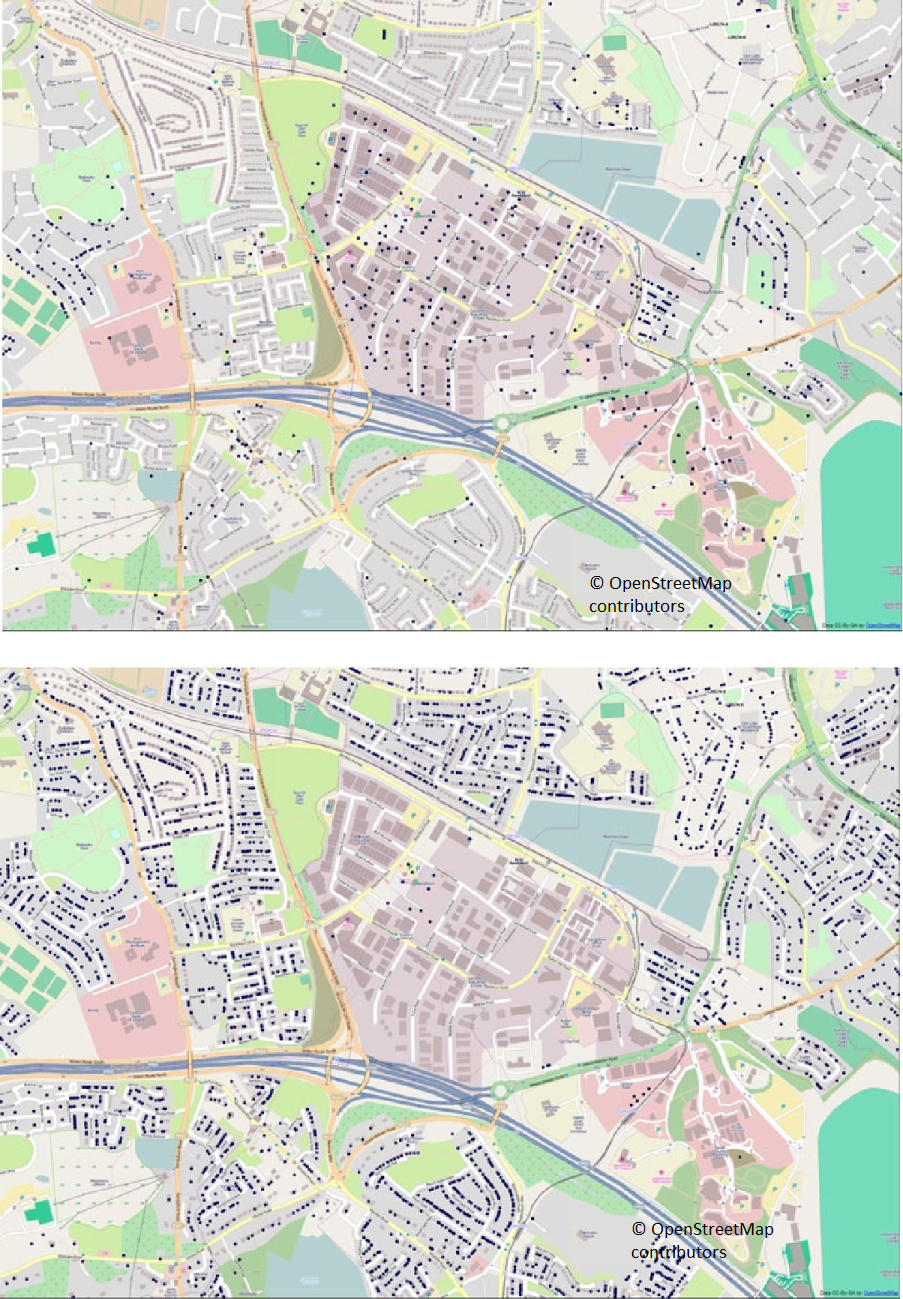
\includegraphics[width=0.99\textwidth, angle=0]{scenarios/figures/dublin0.png}}%
{}
% ------------

% ------------
\createfigure%
{Hourly observed traffic volumes compared to the estimated traffic volumes}%
{Hourly observed traffic volumes (dashed line) compared to the estimated traffic volumes produced by \gls{matsim} using the radiation model (green line) and nearest neighbor model (orange line)}%
{\label{fig:dublin1}}%
{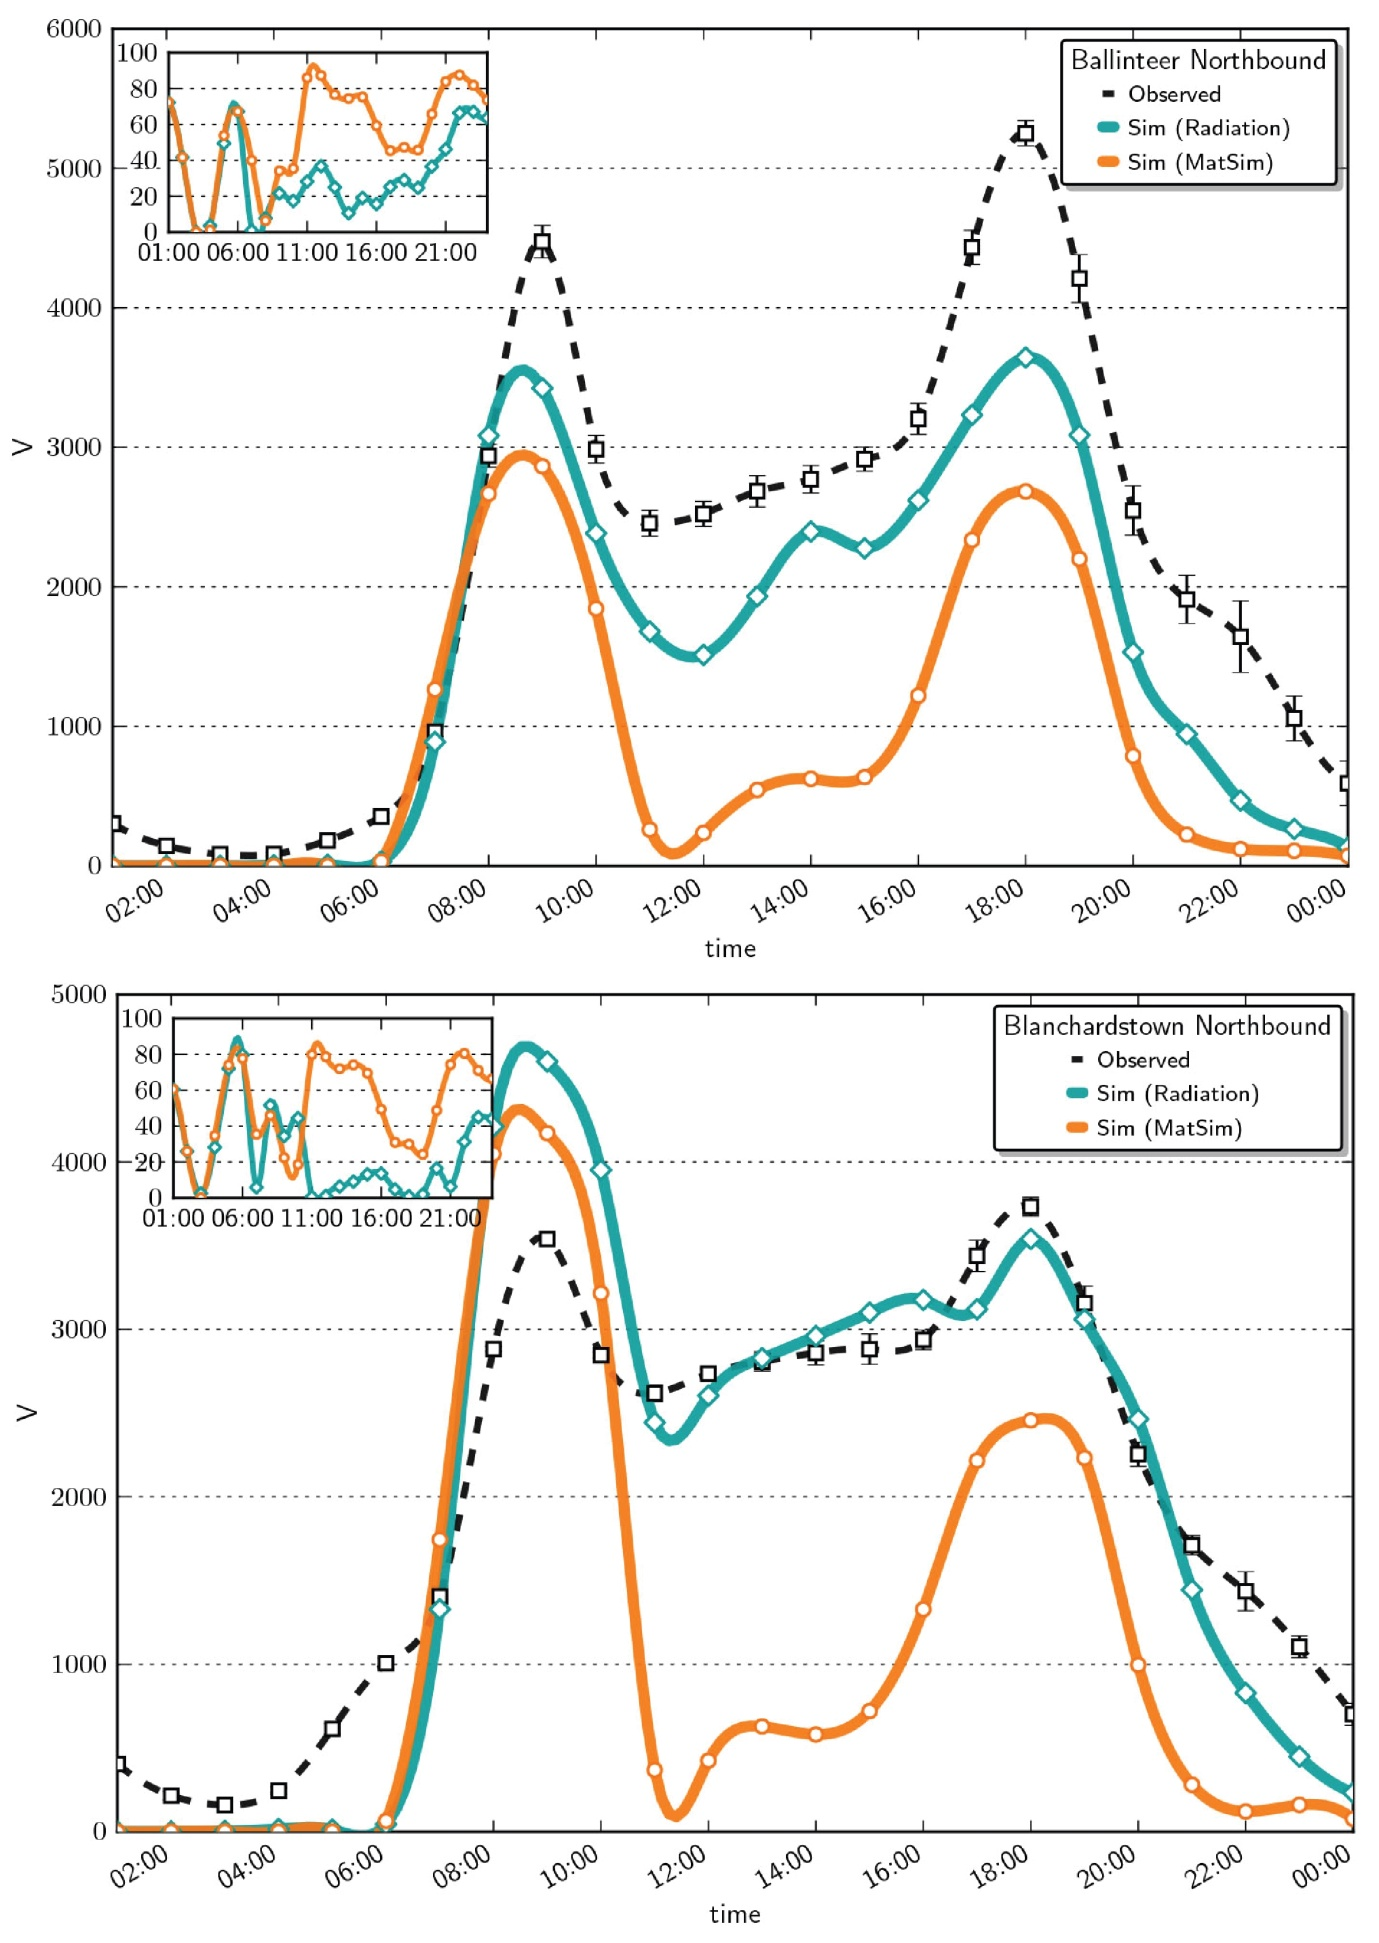
\includegraphics[width=0.99\textwidth, angle=0]{scenarios/figures/dublin1.png}}%
{}
% ------------

% =======================================================================================





